\subsubsubsection{Registrovanje zaposlenog radnika}

\begin{itemize}
    \item Kratak opis:
        \begin{itemize}
            \item Administrator dodaje novog zaposlenog u sistem.
        \end{itemize}
    \item Učesnici:
        \begin{itemize}
            \item Administrator
        \end{itemize}
    \item Preduslovi:
        \begin{itemize}
            \item Administrator poseduje informacije o novozaposlenom.
        \end{itemize}
    \item Postuslovi:
        \begin{itemize}
            \item Novi zaposleni je dodat u sistem i dobio je svoj lični nalog. Podaci su uspešno sačuvani u bazi podataka.
        \end{itemize}
    \item Osnovni tok:
        \begin{enumerate}
         \item Administrator otvara formu za unos podataka.
         \item Administrator vrši validaciju podataka.
         \item Administrator bira vrstu zaposlenog: koordinator, magacioner, dostavljač.
         \item Administrator unosi neophodne podatke i bira opciju ``Dodaj zaposlenog''.
         \item Sistem čuva unete podatke.
         \item Sistem šalje mejl zaposlenom sa linkom za početno pristupanje nalogu.
         \item Administrator putem telefonskog poziva proverava sa zaposlenim da li je dobio mejl za pristup nalogu.
         \item Administrator unosi da je zaposleni dobio mejl i zatvara formu za unos podataka.
        \end{enumerate}
    \item Alternativni tok:
        \begin{itemize}
            \item[2.a] Administrator je uočio nepravilnost u prikupljenim podacima. Administrator kontaktira zaposlenog kako bi dobio ispravne podatke i ispravio ih u formi. Proces se nastavlja u 2. koraku osnovnog toka.
            \item[7.a] Zaposleni nije dobio mejl za pristupanje svom nalogu. Administrator zahteva od sistema da ponovo pošalje mejl. Proces se nastavlja u 6. koraku osnovnog toka.
            \item[7.b] Administrator ne može da stupi u kontakt sa zaposlenim. Čuva se trenutno stanje i privremeno se prekida slučaj upotrebe. Nakon određenog vremena slučaj upotrebe se nastavlja ponovnim zvanjem zaposlenog tj. od 7. koraka osnovnog toka.
        \end{itemize}
    \item Dodatne informacije:
        \begin{itemize}
            \item Podaci koji su neophodni za registraciju novog zaposlenog su: ime, prezime, mejl, telefon, jmbg.
        \end{itemize}
\end{itemize}

\begin{figure}[H]
\begin{center}
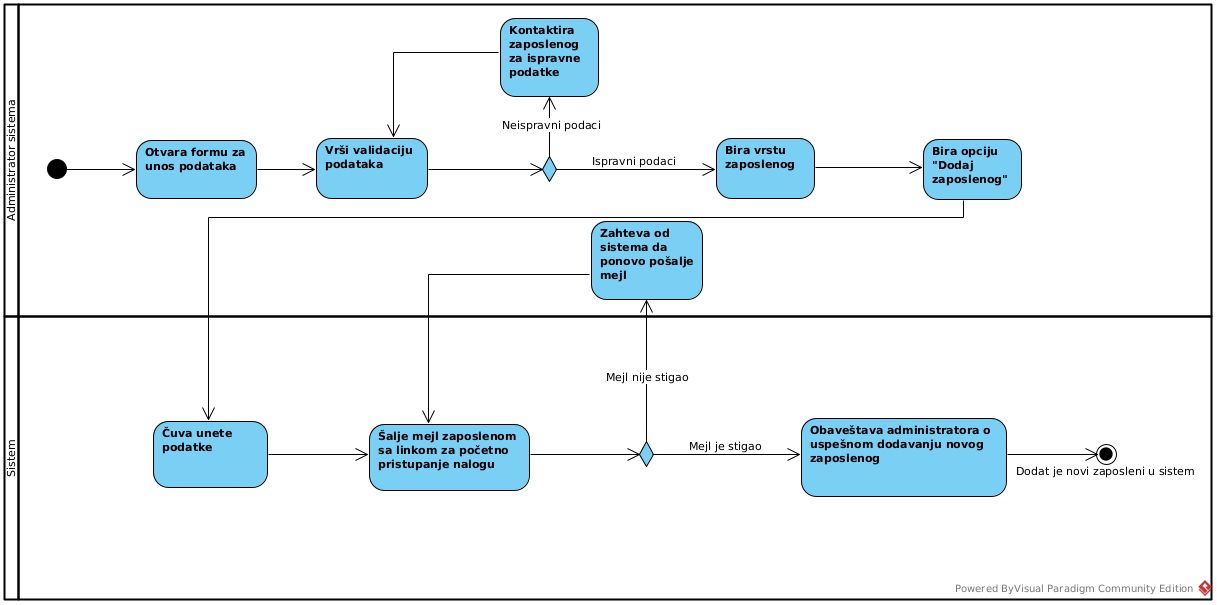
\includegraphics[width=\textwidth]{Pictures/activity_employee_registration.png}
\end{center}
    \caption{Dijagram aktivnosti registrovanje novog zaposlenog radnika}
\label{fig:ActivityEmployeeRegistration}
\end{figure}
